\documentclass[tikz,border=5pt]{standalone}
\usepackage{pgfplots}
\pgfplotsset{compat=1.18}

\definecolor{myCol}{HTML}{5481B0}

\begin{document}
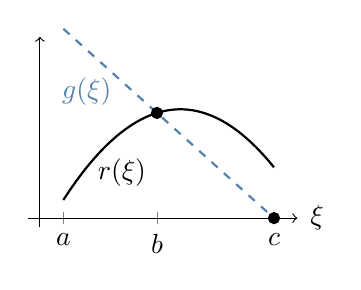
\begin{tikzpicture}
\begin{axis}[
    width=5cm,
    height=4cm,
    axis lines=middle,
    axis line style={->},
    xlabel={$\xi$},
    ylabel={},
    xlabel style={
        at={(axis description cs:0.95,0.05)},
        anchor=west,
        xshift=6pt
    },
    ylabel style={
        at={(axis description cs:0.05,0.95)},
        anchor=south,
        yshift=6pt
    },
    xmin=-0.1, xmax=2.2,
    ymin=-0.1, ymax=2,
    xtick={0.2,1,2},
    xticklabels={$a$,$b$,$c$},
    ytick=\empty,
    domain=0.2:2,
    samples=200,
    clip=false,
    legend style={draw=none, at={(0.02,0.95)}, anchor=west}
]

% Concave function r
\addplot[thick, black,domain=0.2:2]
    {- (x-1.2)^2 + 1.2};
%\addlegendentry{$r(\xi)$}

% Affine function g (secant through b and c)
\addplot[thick, myCol, dashed, domain=0.2:2]
    {(- (1-1.2)^2 + 1.2)
     + (0 - (- (1-1.2)^2 + 1.2))*(x-1)};
%\addlegendentry{$f(\xi)$}

% Points a, b, c
\addplot[only marks, mark=*, black] coordinates {
    % (0.2,{-(0.2-1.2)^2+1.2})
    (1,{-(1-1.2)^2+1.2})
    (2,{0})
};

% Inequality annotations
\node[myCol] at (axis cs:0.4,1.4) {$g(\xi)$};
\node at (axis cs:0.7,0.5) {$r(\xi)$};

\end{axis}
\end{tikzpicture}
\end{document}
